% Options for packages loaded elsewhere
\PassOptionsToPackage{unicode}{hyperref}
\PassOptionsToPackage{hyphens}{url}
%
\documentclass[
]{article}
\usepackage{lmodern}
\usepackage{amsmath}
\usepackage{ifxetex,ifluatex}
\ifnum 0\ifxetex 1\fi\ifluatex 1\fi=0 % if pdftex
  \usepackage[T1]{fontenc}
  \usepackage[utf8]{inputenc}
  \usepackage{textcomp} % provide euro and other symbols
  \usepackage{amssymb}
\else % if luatex or xetex
  \usepackage{unicode-math}
  \defaultfontfeatures{Scale=MatchLowercase}
  \defaultfontfeatures[\rmfamily]{Ligatures=TeX,Scale=1}
\fi
% Use upquote if available, for straight quotes in verbatim environments
\IfFileExists{upquote.sty}{\usepackage{upquote}}{}
\IfFileExists{microtype.sty}{% use microtype if available
  \usepackage[]{microtype}
  \UseMicrotypeSet[protrusion]{basicmath} % disable protrusion for tt fonts
}{}
\makeatletter
\@ifundefined{KOMAClassName}{% if non-KOMA class
  \IfFileExists{parskip.sty}{%
    \usepackage{parskip}
  }{% else
    \setlength{\parindent}{0pt}
    \setlength{\parskip}{6pt plus 2pt minus 1pt}}
}{% if KOMA class
  \KOMAoptions{parskip=half}}
\makeatother
\usepackage{xcolor}
\IfFileExists{xurl.sty}{\usepackage{xurl}}{} % add URL line breaks if available
\IfFileExists{bookmark.sty}{\usepackage{bookmark}}{\usepackage{hyperref}}
\hypersetup{
  pdftitle={format\_data},
  pdfauthor={Dan Weinberger},
  hidelinks,
  pdfcreator={LaTeX via pandoc}}
\urlstyle{same} % disable monospaced font for URLs
\usepackage[margin=1in]{geometry}
\usepackage{graphicx}
\makeatletter
\def\maxwidth{\ifdim\Gin@nat@width>\linewidth\linewidth\else\Gin@nat@width\fi}
\def\maxheight{\ifdim\Gin@nat@height>\textheight\textheight\else\Gin@nat@height\fi}
\makeatother
% Scale images if necessary, so that they will not overflow the page
% margins by default, and it is still possible to overwrite the defaults
% using explicit options in \includegraphics[width, height, ...]{}
\setkeys{Gin}{width=\maxwidth,height=\maxheight,keepaspectratio}
% Set default figure placement to htbp
\makeatletter
\def\fps@figure{htbp}
\makeatother
\setlength{\emergencystretch}{3em} % prevent overfull lines
\providecommand{\tightlist}{%
  \setlength{\itemsep}{0pt}\setlength{\parskip}{0pt}}
\setcounter{secnumdepth}{-\maxdimen} % remove section numbering
\usepackage{booktabs}
\usepackage{longtable}
\usepackage{array}
\usepackage{multirow}
\usepackage{wrapfig}
\usepackage{float}
\usepackage{colortbl}
\usepackage{pdflscape}
\usepackage{tabu}
\usepackage{threeparttable}
\usepackage{threeparttablex}
\usepackage[normalem]{ulem}
\usepackage{makecell}
\usepackage{xcolor}
\ifluatex
  \usepackage{selnolig}  % disable illegal ligatures
\fi

\title{format\_data}
\author{Dan Weinberger}
\date{5/25/2021}

\begin{document}
\maketitle

\hypertarget{instructions-to-get-survey-data}{%
\subsection{INSTRUCTIONS TO GET SURVEY
DATA}\label{instructions-to-get-survey-data}}

\begin{enumerate}
\def\labelenumi{\arabic{enumi}.}
\tightlist
\item
  Go to Yale qualtrics site
\item
  Navigate to Intake questionaire.
\item
  Download data as .xlsx
\item
  Repeat for fortnightly survey
\end{enumerate}

ID 6.1 Saliva was very low under 100 ul.

ID 5.6 qpcr LytA -piaB was ran in plate A155\_scope\_2021\_06\_02 .The
issue was the label: FIXED 5.5 to 5.6

ID 62.2,63.2 samples were picked up 1 month after .We didn't see any
growth after incubation 37 degree over night

ID 20.5 - 21.5 to verify

\begin{verbatim}
## New names:
## * `` -> ...36
\end{verbatim}

\begin{verbatim}
## [1] "A143_scope_2021_05_11.xlsx"
## [1] "A144_scope_2021_05_12_DC.xlsx"
## [1] "A145_scope_2021_05_04.xlsx"
## [1] "A146_scope_2021_05_17.xlsx"
## [1] "A146_scope_2021_06_03 lyta_DC.xlsx"
## [1] "A147_scope_2021_05_17 piaB.xlsx"
## [1] "A148_SCOPE 1_2021_11_30_lyta_repeat AT,SD.xlsx"
## [1] "A148_scope_2021_05_19 piaB.xlsx"
## [1] "A148_scope_2021_05_27_repeatedwithnewlytaprobe_DC.xlsx"
## [1] "A149_scope_2021_05_19_piaB_DC.xlsx"
## [1] "A149_scope_2021_06_09_lytarepeat_DC.pltd.xlsx"
## [1] "A150_scope_2021_05_24_DC.xlsx"
## [1] "A151_scope _2021-06-17_piab_DC_repeat.xlsx"
## [1] "A151_scope_2021_05_29 repeat lyta_DC.xlsx"
## [1] "A153_scope_2021_05_29_DC.xlsx"
## [1] "A154_2021_-06_02_DC.xlsx"
## [1] "A155_2021_06_02_DC.xlsx"
## [1] "A156_scope_2021_06_03_DC.xlsx"
## [1] "A157_scope_2021_06_08 lyta-piaB repeat_DC.xlsx"
\end{verbatim}

\begin{verbatim}
## New names:
## * `` -> ...3
\end{verbatim}

\begin{verbatim}
## [1] "A161-lyta_piab_scope_2021-06-23 pcrd DC.xlsx"
## [1] "A162_SCOPE_2021_12_01_rerun (1).xlsx"
## [1] "A163_SCOPE_2021_09_15_lyta_piab_sso_DC.xlsx"
## [1] "A164_SCOPE_2021_10_01_ext_lyta_piab_validate.xlsx"
## [1] "A165_SCOPE_2021_12_03 (3).xlsx"
## [1] "A197_scope1_2021-12-09 biorad sm.xlsx"
## [1] "S01_SCOPE II_2022.xls"
## [1] "S15_scope_2022-11-23 _xlytA_piaB.xlsx"
\end{verbatim}

\begin{verbatim}
## Warning: NAs introduced by coercion
\end{verbatim}

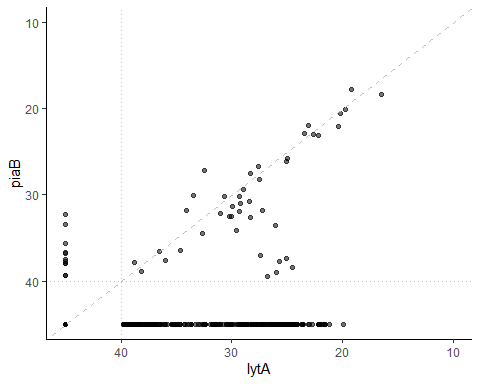
\includegraphics{format-raw_files/figure-latex/unnamed-chunk-2-1.pdf}

\hypertarget{heatmaps}{%
\subsection{Heatmaps}\label{heatmaps}}

piaB

\includegraphics{format-raw_files/figure-latex/unnamed-chunk-4-1.pdf}
\includegraphics{format-raw_files/figure-latex/unnamed-chunk-4-2.pdf}
\includegraphics{format-raw_files/figure-latex/unnamed-chunk-4-3.pdf}

lytA

\includegraphics{format-raw_files/figure-latex/unnamed-chunk-5-1.pdf}

\begin{verbatim}
## Warning in dev.off(): unable to open TIFF file 'Heat lyta .tiff'
\end{verbatim}

\includegraphics{format-raw_files/figure-latex/unnamed-chunk-5-2.pdf}
\includegraphics{format-raw_files/figure-latex/unnamed-chunk-5-3.pdf}

Contacts

\hypertarget{summary-stats}{%
\subsection{Summary stats}\label{summary-stats}}

\begin{verbatim}
## [1] 95
\end{verbatim}

\begin{verbatim}
## [1] 48
\end{verbatim}

\begin{verbatim}
## [1] 567
\end{verbatim}

\begin{verbatim}
## [1] 52
\end{verbatim}

\begin{verbatim}
## [1] 0.09171076
\end{verbatim}

\begin{verbatim}
## [1] 154
\end{verbatim}

\begin{verbatim}
## [1] 0.2716049
\end{verbatim}

\begin{verbatim}
## [1] 28
\end{verbatim}

\begin{verbatim}
## [1] 20
\end{verbatim}

\begin{verbatim}
## New names:
## * `` -> ...1
## * `` -> ...13
## * `` -> ...14
## * `` -> ...15
\end{verbatim}

\begin{verbatim}
## [1] 71.02105
\end{verbatim}

\begin{verbatim}
## [1] 60 86
\end{verbatim}

\hypertarget{merge-in-results-with-master-file}{%
\subsection{Merge in results with master
file}\label{merge-in-results-with-master-file}}

--To do: -harmonize column names between fortnightly and initial
questionaire so we can merge -Fix dates -Check missing visitNs

Intake questionaire

\begin{verbatim}
## New names:
## * `Where did you receive this vaccine? - Selected Choice` -> `Where did you receive this vaccine? - Selected Choice...31`
## * `Where did you receive this vaccine? - Doctor's Office (Name of Provider) - Text` -> `Where did you receive this vaccine? - Doctor's Office (Name of Provider) - Text...32`
## * `Where did you receive this vaccine? - Other - Text` -> `Where did you receive this vaccine? - Other - Text...33`
## * `Where did you receive this vaccine? - Selected Choice` -> `Where did you receive this vaccine? - Selected Choice...55`
## * `Where did you receive this vaccine? - Doctor's Office (Name of Provider) - Text` -> `Where did you receive this vaccine? - Doctor's Office (Name of Provider) - Text...56`
## * ...
## New names:
## * `Where did you receive this vaccine? - Selected Choice` -> `Where did you receive this vaccine? - Selected Choice...31`
## * `Where did you receive this vaccine? - Doctor's Office (Name of Provider) - Text` -> `Where did you receive this vaccine? - Doctor's Office (Name of Provider) - Text...32`
## * `Where did you receive this vaccine? - Other - Text` -> `Where did you receive this vaccine? - Other - Text...33`
## * `Where did you receive this vaccine? - Selected Choice` -> `Where did you receive this vaccine? - Selected Choice...55`
## * `Where did you receive this vaccine? - Doctor's Office (Name of Provider) - Text` -> `Where did you receive this vaccine? - Doctor's Office (Name of Provider) - Text...56`
## * ...
\end{verbatim}

Fortnightly questionnaire and intake cleaning\ldots do not run each time

read in newly entered surveys

\begin{verbatim}
## Warning: NAs introduced by coercion
\end{verbatim}

\begin{verbatim}
## Warning in as.Date(as.numeric(q2$visit_date), origin = "1900-01-01"): NAs
## introduced by coercion
\end{verbatim}

\begin{verbatim}
## Warning in as.Date(as.numeric(q2$visit_date_cleaned), origin = "1900-01-01"):
## NAs introduced by coercion
\end{verbatim}

\begin{verbatim}
## Using visitN as value column: use value.var to override.
\end{verbatim}

\begin{verbatim}
## Warning: 17 failed to parse.
\end{verbatim}

\begin{verbatim}
## New names:
## * `` -> ...1
## * `` -> ...13
## * `` -> ...14
## * `` -> ...15
\end{verbatim}

heat map of contacts

\includegraphics{format-raw_files/figure-latex/unnamed-chunk-12-1.pdf}
\includegraphics{format-raw_files/figure-latex/unnamed-chunk-12-2.pdf}
\includegraphics{format-raw_files/figure-latex/unnamed-chunk-12-3.pdf}

\begin{verbatim}
## TableGrob (1 x 2) "arrange": 2 grobs
##   z     cells    name           grob
## 1 1 (1-1,1-1) arrange gtable[layout]
## 2 2 (1-1,2-2) arrange gtable[layout]
\end{verbatim}

\includegraphics{format-raw_files/figure-latex/unnamed-chunk-13-1.pdf}

Do you usually have contact with children?

\begin{tabular}[t]{lllll}
\toprule
  & NA & No & Yes & Overall\\
\midrule
 & (N=13) & (N=312) & (N=199) & (N=584)\\
\addlinespace[0.3em]
\multicolumn{5}{l}{\textbf{piab\_pos}}\\
\hspace{1em}0 & 12 (92.3\%) & 286 (91.7\%) & 162 (81.4\%) & 515 (88.2\%)\\
\hspace{1em}1 & 1 (7.7\%) & 19 (6.1\%) & 27 (13.6\%) & 52 (8.9\%)\\
\hspace{1em}Missing & 0 (0\%) & 7 (2.2\%) & 10 (5.0\%) & 17 (2.9\%)\\
\bottomrule
\end{tabular}

Contact \textless5 y olds

\begin{tabular}[t]{lllll}
\toprule
  & No & Not answered & Yes & Overall\\
\midrule
 & (N=412) & (N=90) & (N=82) & (N=584)\\
\addlinespace[0.3em]
\multicolumn{5}{l}{\textbf{piab\_pos}}\\
\hspace{1em}0 & 367 (89.1\%) & 82 (91.1\%) & 66 (80.5\%) & 515 (88.2\%)\\
\hspace{1em}1 & 33 (8.0\%) & 6 (6.7\%) & 13 (15.9\%) & 52 (8.9\%)\\
\hspace{1em}Missing & 12 (2.9\%) & 2 (2.2\%) & 3 (3.7\%) & 17 (2.9\%)\\
\bottomrule
\end{tabular}

How often do you have contact with children?

\begin{tabular}[t]{lllllll}
\toprule
  & Daily & Every few days & NA & No & Once or twice a month & Overall\\
\midrule
 & (N=23) & (N=105) & (N=26) & (N=312) & (N=57) & (N=584)\\
\addlinespace[0.3em]
\multicolumn{7}{l}{\textbf{piab\_pos}}\\
\hspace{1em}0 & 20 (87.0\%) & 83 (79.0\%) & 24 (92.3\%) & 286 (91.7\%) & 47 (82.5\%) & 515 (88.2\%)\\
\hspace{1em}1 & 3 (13.0\%) & 17 (16.2\%) & 2 (7.7\%) & 19 (6.1\%) & 5 (8.8\%) & 52 (8.9\%)\\
\hspace{1em}Missing & 0 (0\%) & 5 (4.8\%) & 0 (0\%) & 7 (2.2\%) & 5 (8.8\%) & 17 (2.9\%)\\
\bottomrule
\end{tabular}

How much contact per day do you have?

\begin{tabular}[t]{llllll}
\toprule
  & <4 hours (morning or afternoon or evening) & 4-8 hours (full day) & 8+ hours (longer day care/overnight) & NA & Overall\\
\midrule
 & (N=131) & (N=52) & (N=16) & (N=296) & (N=584)\\
\addlinespace[0.3em]
\multicolumn{6}{l}{\textbf{piab\_pos}}\\
\hspace{1em}0 & 107 (81.7\%) & 41 (78.8\%) & 13 (81.3\%) & 273 (92.2\%) & 515 (88.2\%)\\
\hspace{1em}1 & 18 (13.7\%) & 7 (13.5\%) & 3 (18.8\%) & 18 (6.1\%) & 52 (8.9\%)\\
\hspace{1em}Missing & 6 (4.6\%) & 4 (7.7\%) & 0 (0\%) & 5 (1.7\%) & 17 (2.9\%)\\
\bottomrule
\end{tabular}

What ages do you have contact with?

\textless12m?

\begin{tabular}[t]{lllll}
\toprule
  & No & Not answered & Yes & Overall\\
\midrule
 & (N=452) & (N=90) & (N=42) & (N=584)\\
\addlinespace[0.3em]
\multicolumn{5}{l}{\textbf{piab\_pos}}\\
\hspace{1em}0 & 397 (87.8\%) & 82 (91.1\%) & 36 (85.7\%) & 515 (88.2\%)\\
\hspace{1em}1 & 41 (9.1\%) & 6 (6.7\%) & 5 (11.9\%) & 52 (8.9\%)\\
\hspace{1em}Missing & 14 (3.1\%) & 2 (2.2\%) & 1 (2.4\%) & 17 (2.9\%)\\
\bottomrule
\end{tabular}

12-23m?

\begin{tabular}[t]{lllll}
\toprule
  & No & Not answered & Yes & Overall\\
\midrule
 & (N=477) & (N=90) & (N=17) & (N=584)\\
\addlinespace[0.3em]
\multicolumn{5}{l}{\textbf{piab\_pos}}\\
\hspace{1em}0 & 421 (88.3\%) & 82 (91.1\%) & 12 (70.6\%) & 515 (88.2\%)\\
\hspace{1em}1 & 44 (9.2\%) & 6 (6.7\%) & 2 (11.8\%) & 52 (8.9\%)\\
\hspace{1em}Missing & 12 (2.5\%) & 2 (2.2\%) & 3 (17.6\%) & 17 (2.9\%)\\
\bottomrule
\end{tabular}

2-5y

\begin{tabular}[t]{lllll}
\toprule
  & No & Not answered & Yes & Overall\\
\midrule
 & (N=455) & (N=90) & (N=39) & (N=584)\\
\addlinespace[0.3em]
\multicolumn{5}{l}{\textbf{piab\_pos}}\\
\hspace{1em}0 & 401 (88.1\%) & 82 (91.1\%) & 32 (82.1\%) & 515 (88.2\%)\\
\hspace{1em}1 & 39 (8.6\%) & 6 (6.7\%) & 7 (17.9\%) & 52 (8.9\%)\\
\hspace{1em}Missing & 15 (3.3\%) & 2 (2.2\%) & 0 (0\%) & 17 (2.9\%)\\
\bottomrule
\end{tabular}

5-10y

\begin{tabular}[t]{lllll}
\toprule
  & No & Not answered & Yes & Overall\\
\midrule
 & (N=406) & (N=90) & (N=88) & (N=584)\\
\addlinespace[0.3em]
\multicolumn{5}{l}{\textbf{piab\_pos}}\\
\hspace{1em}0 & 365 (89.9\%) & 82 (91.1\%) & 68 (77.3\%) & 515 (88.2\%)\\
\hspace{1em}1 & 32 (7.9\%) & 6 (6.7\%) & 14 (15.9\%) & 52 (8.9\%)\\
\hspace{1em}Missing & 9 (2.2\%) & 2 (2.2\%) & 6 (6.8\%) & 17 (2.9\%)\\
\bottomrule
\end{tabular}

more than 10y

\begin{tabular}[t]{lllll}
\toprule
  & No & Not answered & Yes & Overall\\
\midrule
 & (N=427) & (N=90) & (N=67) & (N=584)\\
\addlinespace[0.3em]
\multicolumn{5}{l}{\textbf{piab\_pos}}\\
\hspace{1em}0 & 376 (88.1\%) & 82 (91.1\%) & 57 (85.1\%) & 515 (88.2\%)\\
\hspace{1em}1 & 38 (8.9\%) & 6 (6.7\%) & 8 (11.9\%) & 52 (8.9\%)\\
\hspace{1em}Missing & 13 (3.0\%) & 2 (2.2\%) & 2 (3.0\%) & 17 (2.9\%)\\
\bottomrule
\end{tabular}

Have you taken part in any social activities or outings during the past
two weeks?

\begin{tabular}[t]{lllll}
\toprule
  & NA & No & Yes & Overall\\
\midrule
 & (N=86) & (N=187) & (N=245) & (N=584)\\
\addlinespace[0.3em]
\multicolumn{5}{l}{\textbf{piab\_pos}}\\
\hspace{1em}0 & 73 (84.9\%) & 164 (87.7\%) & 219 (89.4\%) & 515 (88.2\%)\\
\hspace{1em}1 & 7 (8.1\%) & 18 (9.6\%) & 20 (8.2\%) & 52 (8.9\%)\\
\hspace{1em}Missing & 6 (7.0\%) & 5 (2.7\%) & 6 (2.4\%) & 17 (2.9\%)\\
\bottomrule
\end{tabular}

What sorts of activities have you participated in? - Selected Choice

\begin{tabular}[t]{lllllllll}
\toprule
  & Activities at community centers & Activities with family & Activities with friends & Fitness activities & NA & No & Other & Overall\\
\midrule
 & (N=8) & (N=74) & (N=36) & (N=10) & (N=90) & (N=187) & (N=113) & (N=584)\\
\addlinespace[0.3em]
\multicolumn{9}{l}{\textbf{piab\_pos}}\\
\hspace{1em}0 & 8 (100\%) & 60 (81.1\%) & 35 (97.2\%) & 10 (100\%) & 77 (85.6\%) & 164 (87.7\%) & 102 (90.3\%) & 515 (88.2\%)\\
\hspace{1em}1 & 0 (0\%) & 11 (14.9\%) & 1 (2.8\%) & 0 (0\%) & 7 (7.8\%) & 18 (9.6\%) & 8 (7.1\%) & 52 (8.9\%)\\
\hspace{1em}Missing & 0 (0\%) & 3 (4.1\%) & 0 (0\%) & 0 (0\%) & 6 (6.7\%) & 5 (2.7\%) & 3 (2.7\%) & 17 (2.9\%)\\
\bottomrule
\end{tabular}

\hypertarget{current-symptoms}{%
\subsection{Current Symptoms}\label{current-symptoms}}

Cough?

\begin{tabular}[t]{lllll}
\toprule
  & NA & No & Yes & Overall\\
\midrule
 & (N=2) & (N=508) & (N=13) & (N=584)\\
\addlinespace[0.3em]
\multicolumn{5}{l}{\textbf{piab\_pos}}\\
\hspace{1em}0 & 2 (100\%) & 447 (88.0\%) & 10 (76.9\%) & 515 (88.2\%)\\
\hspace{1em}1 & 0 (0\%) & 44 (8.7\%) & 3 (23.1\%) & 52 (8.9\%)\\
\hspace{1em}Missing & 0 (0\%) & 17 (3.3\%) & 0 (0\%) & 17 (2.9\%)\\
\bottomrule
\end{tabular}

Runny Nose?

\begin{tabular}[t]{lllll}
\toprule
  & NA & No & Yes & Overall\\
\midrule
 & (N=1) & (N=503) & (N=19) & (N=584)\\
\addlinespace[0.3em]
\multicolumn{5}{l}{\textbf{piab\_pos}}\\
\hspace{1em}0 & 1 (100\%) & 442 (87.9\%) & 16 (84.2\%) & 515 (88.2\%)\\
\hspace{1em}1 & 0 (0\%) & 44 (8.7\%) & 3 (15.8\%) & 52 (8.9\%)\\
\hspace{1em}Missing & 0 (0\%) & 17 (3.4\%) & 0 (0\%) & 17 (2.9\%)\\
\bottomrule
\end{tabular}

Fever?

\begin{tabular}[t]{llll}
\toprule
  & NA & No & Overall\\
\midrule
 & (N=4) & (N=519) & (N=584)\\
\addlinespace[0.3em]
\multicolumn{4}{l}{\textbf{piab\_pos}}\\
\hspace{1em}0 & 3 (75.0\%) & 456 (87.9\%) & 515 (88.2\%)\\
\hspace{1em}1 & 0 (0\%) & 47 (9.1\%) & 52 (8.9\%)\\
\hspace{1em}Missing & 1 (25.0\%) & 16 (3.1\%) & 17 (2.9\%)\\
\bottomrule
\end{tabular}

Sore throat?

\begin{tabular}[t]{lllll}
\toprule
  & NA & No & Yes & Overall\\
\midrule
 & (N=1) & (N=521) & (N=1) & (N=584)\\
\addlinespace[0.3em]
\multicolumn{5}{l}{\textbf{piab\_pos}}\\
\hspace{1em}0 & 1 (100\%) & 457 (87.7\%) & 1 (100\%) & 515 (88.2\%)\\
\hspace{1em}1 & 0 (0\%) & 47 (9.0\%) & 0 (0\%) & 52 (8.9\%)\\
\hspace{1em}Missing & 0 (0\%) & 17 (3.3\%) & 0 (0\%) & 17 (2.9\%)\\
\bottomrule
\end{tabular}

Nasal?

\begin{tabular}[t]{lllll}
\toprule
  & NA & No & Yes & Overall\\
\midrule
 & (N=1) & (N=504) & (N=18) & (N=584)\\
\addlinespace[0.3em]
\multicolumn{5}{l}{\textbf{piab\_pos}}\\
\hspace{1em}0 & 1 (100\%) & 442 (87.7\%) & 16 (88.9\%) & 515 (88.2\%)\\
\hspace{1em}1 & 0 (0\%) & 45 (8.9\%) & 2 (11.1\%) & 52 (8.9\%)\\
\hspace{1em}Missing & 0 (0\%) & 17 (3.4\%) & 0 (0\%) & 17 (2.9\%)\\
\bottomrule
\end{tabular}

\hypertarget{pneumooccal-vaccination}{%
\subsection{Pneumooccal vaccination}\label{pneumooccal-vaccination}}

\begin{tabular}[t]{llll}
\toprule
  & No & Yes & Overall\\
\midrule
 & (N=115) & (N=317) & (N=584)\\
\addlinespace[0.3em]
\multicolumn{4}{l}{\textbf{piab\_pos}}\\
\hspace{1em}0 & 104 (90.4\%) & 282 (89.0\%) & 515 (88.2\%)\\
\hspace{1em}1 & 7 (6.1\%) & 25 (7.9\%) & 52 (8.9\%)\\
\hspace{1em}Missing & 4 (3.5\%) & 10 (3.2\%) & 17 (2.9\%)\\
\bottomrule
\end{tabular}

\#\#COVID History

\begin{tabular}[t]{lllll}
\toprule
  & No, it was negative & Not tested & Yes, it was positive & Overall\\
\midrule
 & (N=292) & (N=98) & (N=44) & (N=584)\\
\addlinespace[0.3em]
\multicolumn{5}{l}{\textbf{piab\_pos}}\\
\hspace{1em}0 & 261 (89.4\%) & 91 (92.9\%) & 38 (86.4\%) & 515 (88.2\%)\\
\hspace{1em}1 & 22 (7.5\%) & 2 (2.0\%) & 6 (13.6\%) & 52 (8.9\%)\\
\hspace{1em}Missing & 9 (3.1\%) & 5 (5.1\%) & 0 (0\%) & 17 (2.9\%)\\
\bottomrule
\end{tabular}

\hypertarget{ethnicity}{%
\subsection{Ethnicity}\label{ethnicity}}

\begin{tabular}[t]{llllllll}
\toprule
  & Asian & Asian,Unknown/Other & Black or African American & Unknown/Other & White & White,Unknown/Other & Overall\\
\midrule
 & (N=6) & (N=12) & (N=18) & (N=12) & (N=386) & (N=6) & (N=584)\\
\addlinespace[0.3em]
\multicolumn{8}{l}{\textbf{piab\_pos}}\\
\hspace{1em}0 & 6 (100\%) & 12 (100\%) & 18 (100\%) & 10 (83.3\%) & 343 (88.9\%) & 5 (83.3\%) & 515 (88.2\%)\\
\hspace{1em}1 & 0 (0\%) & 0 (0\%) & 0 (0\%) & 2 (16.7\%) & 29 (7.5\%) & 1 (16.7\%) & 52 (8.9\%)\\
\hspace{1em}Missing & 0 (0\%) & 0 (0\%) & 0 (0\%) & 0 (0\%) & 14 (3.6\%) & 0 (0\%) & 17 (2.9\%)\\
\bottomrule
\end{tabular}

\hypertarget{education-level}{%
\subsection{Education level}\label{education-level}}

\#Medications Immune meds

\begin{tabular}[t]{lllll}
\toprule
  & Don't know & No & Yes & Overall\\
\midrule
 & (N=12) & (N=399) & (N=29) & (N=584)\\
\addlinespace[0.3em]
\multicolumn{5}{l}{\textbf{piab\_pos}}\\
\hspace{1em}0 & 12 (100\%) & 356 (89.2\%) & 26 (89.7\%) & 515 (88.2\%)\\
\hspace{1em}1 & 0 (0\%) & 29 (7.3\%) & 3 (10.3\%) & 52 (8.9\%)\\
\hspace{1em}Missing & 0 (0\%) & 14 (3.5\%) & 0 (0\%) & 17 (2.9\%)\\
\bottomrule
\end{tabular}

Asthma meds

\begin{tabular}[t]{lllll}
\toprule
  & Don't know & No & Yes & Overall\\
\midrule
 & (N=5) & (N=403) & (N=12) & (N=584)\\
\addlinespace[0.3em]
\multicolumn{5}{l}{\textbf{piab\_pos}}\\
\hspace{1em}0 & 4 (80.0\%) & 359 (89.1\%) & 11 (91.7\%) & 515 (88.2\%)\\
\hspace{1em}1 & 1 (20.0\%) & 30 (7.4\%) & 1 (8.3\%) & 52 (8.9\%)\\
\hspace{1em}Missing & 0 (0\%) & 14 (3.5\%) & 0 (0\%) & 17 (2.9\%)\\
\bottomrule
\end{tabular}

Recent Antibiotics

\begin{tabular}[t]{lllll}
\toprule
  & NA & No & Yes & Overall\\
\midrule
 & (N=5) & (N=489) & (N=28) & (N=584)\\
\addlinespace[0.3em]
\multicolumn{5}{l}{\textbf{piab\_pos}}\\
\hspace{1em}0 & 4 (80.0\%) & 429 (87.7\%) & 25 (89.3\%) & 515 (88.2\%)\\
\hspace{1em}1 & 0 (0\%) & 46 (9.4\%) & 1 (3.6\%) & 52 (8.9\%)\\
\hspace{1em}Missing & 1 (20.0\%) & 14 (2.9\%) & 2 (7.1\%) & 17 (2.9\%)\\
\bottomrule
\end{tabular}

\hypertarget{seasonality}{%
\section{Seasonality}\label{seasonality}}

\begin{verbatim}
## Warning in table1.formula(~piab_pos | month, data = e3): Terms to the right
## of '|' in formula 'x' define table columns and are expected to be factors with
## meaningful labels.
\end{verbatim}

\begin{tabular}[t]{lllllllllllll}
\toprule
  & 1 & 2 & 3 & 4 & 5 & 6 & 7 & 8 & 10 & 11 & 12 & Overall\\
\midrule
 & (N=103) & (N=117) & (N=119) & (N=48) & (N=25) & (N=33) & (N=10) & (N=4) & (N=5) & (N=7) & (N=48) & (N=584)\\
\addlinespace[0.3em]
\multicolumn{13}{l}{\textbf{piab\_pos}}\\
\hspace{1em}0 & 91 (88.3\%) & 110 (94.0\%) & 106 (89.1\%) & 44 (91.7\%) & 22 (88.0\%) & 24 (72.7\%) & 7 (70.0\%) & 4 (100\%) & 5 (100\%) & 5 (71.4\%) & 39 (81.3\%) & 515 (88.2\%)\\
\hspace{1em}1 & 12 (11.7\%) & 7 (6.0\%) & 10 (8.4\%) & 3 (6.3\%) & 1 (4.0\%) & 5 (15.2\%) & 1 (10.0\%) & 0 (0\%) & 0 (0\%) & 2 (28.6\%) & 5 (10.4\%) & 52 (8.9\%)\\
\hspace{1em}Missing & 0 (0\%) & 0 (0\%) & 3 (2.5\%) & 1 (2.1\%) & 2 (8.0\%) & 4 (12.1\%) & 2 (20.0\%) & 0 (0\%) & 0 (0\%) & 0 (0\%) & 4 (8.3\%) & 17 (2.9\%)\\
\bottomrule
\end{tabular}

\hypertarget{recent-vaccine-receipt-note-many-missing}{%
\subsection{Recent Vaccine receipt (note many
missing)}\label{recent-vaccine-receipt-note-many-missing}}

\begin{tabular}[t]{llllll}
\toprule
  & Flu vaccine & NA & Other vaccine, describe: & Pneumonia vaccine & Overall\\
\midrule
 & (N=1) & (N=353) & (N=132) & (N=1) & (N=584)\\
\addlinespace[0.3em]
\multicolumn{6}{l}{\textbf{piab\_pos}}\\
\hspace{1em}0 & 1 (100\%) & 309 (87.5\%) & 120 (90.9\%) & 1 (100\%) & 515 (88.2\%)\\
\hspace{1em}1 & 0 (0\%) & 32 (9.1\%) & 11 (8.3\%) & 0 (0\%) & 52 (8.9\%)\\
\hspace{1em}Missing & 0 (0\%) & 12 (3.4\%) & 1 (0.8\%) & 0 (0\%) & 17 (2.9\%)\\
\bottomrule
\end{tabular}

Simple model

\begin{verbatim}
## 
## Call:
## glm(formula = piab_pos ~ child_contact_u12m + child_contact_13_23m + 
##     child_contact_24_59m + child_contact_5_10y + child_contact_over10y, 
##     family = binomial(link = "log"), data = e3[e3$child_contact_13_23m != 
##         "Not answered", ])
## 
## Deviance Residuals: 
##     Min       1Q   Median       3Q      Max  
## -0.8062  -0.4467  -0.3974  -0.3974   2.2779  
## 
## Coefficients:
##                          Estimate Std. Error z value Pr(>|z|)    
## (Intercept)              -2.57809    0.18373 -14.032   <2e-16 ***
## child_contact_u12mYes    -0.01626    0.45656  -0.036    0.972    
## child_contact_13_23mYes   0.31328    0.64175   0.488    0.625    
## child_contact_24_59mYes   0.34120    0.42491   0.803    0.422    
## child_contact_5_10yYes    0.64162    0.33844   1.896    0.058 .  
## child_contact_over10yYes  0.24012    0.36233   0.663    0.508    
## ---
## Signif. codes:  0 '***' 0.001 '**' 0.01 '*' 0.05 '.' 0.1 ' ' 1
## 
## (Dispersion parameter for binomial family taken to be 1)
## 
##     Null deviance: 303.00  on 478  degrees of freedom
## Residual deviance: 296.14  on 473  degrees of freedom
##   (15 observations deleted due to missingness)
## AIC: 308.14
## 
## Number of Fisher Scoring iterations: 7
\end{verbatim}

\begin{verbatim}
## 
## Call:
## glm(formula = piab_pos ~ child_contact_24_59m, family = binomial(link = "log"), 
##     data = e3[e3$child_contact_13_23m != "Not answered", ])
## 
## Deviance Residuals: 
##     Min       1Q   Median       3Q      Max  
## -0.6290  -0.4308  -0.4308  -0.4308   2.2015  
## 
## Coefficients:
##                         Estimate Std. Error z value Pr(>|z|)    
## (Intercept)              -2.4232     0.1529 -15.852   <2e-16 ***
## child_contact_24_59mYes   0.7056     0.3749   1.882   0.0599 .  
## ---
## Signif. codes:  0 '***' 0.001 '**' 0.01 '*' 0.05 '.' 0.1 ' ' 1
## 
## (Dispersion parameter for binomial family taken to be 1)
## 
##     Null deviance: 303.00  on 478  degrees of freedom
## Residual deviance: 300.15  on 477  degrees of freedom
##   (15 observations deleted due to missingness)
## AIC: 304.15
## 
## Number of Fisher Scoring iterations: 6
\end{verbatim}

There are some survey results missing. We lose information for these
people. But we know their child contacts at other time points so can
infer

\begin{verbatim}
## 
## Call:
## glm(formula = piab_pos ~ any_contact_u12m + any_contact_13_23m + 
##     any_contact_24_59m + any_contact_5_10y + any_contact_over_10y, 
##     family = binomial(link = "logit"), data = e3_filled)
## 
## Deviance Residuals: 
##     Min       1Q   Median       3Q      Max  
## -0.8501  -0.4348  -0.3146  -0.3146   2.4620  
## 
## Coefficients:
##                      Estimate Std. Error z value Pr(>|z|)    
## (Intercept)          -2.98128    0.24779 -12.032  < 2e-16 ***
## any_contact_u12m      0.38731    0.39454   0.982  0.32626    
## any_contact_13_23m   -0.09069    0.48724  -0.186  0.85234    
## any_contact_24_59m    0.39925    0.41441   0.963  0.33535    
## any_contact_5_10y     1.08035    0.33576   3.218  0.00129 ** 
## any_contact_over_10y  0.37318    0.33718   1.107  0.26839    
## ---
## Signif. codes:  0 '***' 0.001 '**' 0.01 '*' 0.05 '.' 0.1 ' ' 1
## 
## (Dispersion parameter for binomial family taken to be 1)
## 
##     Null deviance: 347.55  on 566  degrees of freedom
## Residual deviance: 323.93  on 561  degrees of freedom
##   (17 observations deleted due to missingness)
## AIC: 335.93
## 
## Number of Fisher Scoring iterations: 5
\end{verbatim}

\end{document}
